\section{Sprint 0: Preparación y planificación del proyecto}
El objetivo de este sprint es preparar al proyecto desde una perspectiva tecnológica, metodológica y organizativa, antes de comenzar el desarrollo, para así facilitar la preparación y la puesta en marcha de cada sprint.

Muchas de las actividades que abarca el Sprint 0 ya fueron descriptas en secciones anteriores de este documento, decisiones como que puesto tomará cada integrante del equipo en la metodología ágil, análisis de la situación actual, relevamiento generales, fueron detalladas de forma extensa con anterioridad.

\subsection{Definición de puestos de trabajo}
En este apartado se detallaran que actividades realizará cada integrante al desarrollar el sistema.

\begin{table}[h]
\begin{center}
\resizebox{\textwidth}{!}{
\begin{tabular}{|l|c|c|c|c|}
	\hline                      & Back-end      & Front-end    & DevOps & Tester     \\
	\hline Canizo, Franco       & \checkmark    &              &               & \checkmark \\
	\hline Manganiello, Michael & \checkmark    &              & \checkmark    & \checkmark \\
	\hline Morales, Yanina      &               &  \checkmark  &               & \checkmark \\
	\hline Terreno, Iván        &               & \checkmark   &               & \checkmark \\
	\hline \textbf{Total}       & \textbf{2}    & \textbf{2}   & \textbf{1}    & \textbf{4} \\
\hline
\end{tabular}
}
\caption{Equipo de trabajo}
\label{equipoDeTrabajo}
\end{center}
\end{table}



\begin{itemize}
	\item \textbf{Back-end:} 
    
   El Back-End es el área que se dedica a la parte lógica de un sitio web, es el encargado de que todo funcione como debería, el back-end es la parte de atrás que de alguna manera no es visible para el usuario ya que no se trata de diseño, o elementos gráficos, se trata de programar las funciones que tendrá un sitio. El Back-End es la programación dura y pura, desde la programación de las funciones del sitio hasta bases de datos e incluso mas.


    Los responsables de esta parte del proyecto usarán \textbf{Flask}, éste es un framework minimalista, caracterizado por su simplicidad y flexibilidad, escrito en Python y basado en la especificación WSGI de Werkzeug y el motor de templates Jinja2. Tiene la licencia BSD.
    
    La elección de esta herramienta está fundada
    \item \textbf{Front-end:}
    
     En diseño de software, el front-end, es la parte del software que interactúa con el o los usuarios y, el back-end, es la parte que procesa la entrada desde el front-end. La separación del sistema en front-ends y back-ends es un tipo de abstracción que ayuda a mantener las diferentes partes del sistema separadas. La idea general es que el front-end sea el responsable de recolectar los datos de entrada del usuario, que pueden ser de muchas y variadas formas, y los transforma ajustándolos a las especificaciones que demanda el back-end para poder procesarlos, devolviendo generalmente una respuesta que el front-end recibe y expone al usuario de una forma entendible.
     
    Los responsables de esta parte del proyecto usarán \textbf{AngularJS}, éste es un framework de JavaScript de código abierto, mantenido por Google, que ayuda con la gestión de lo que se conoce como aplicaciones de una sola página. Su objetivo es aumentar las aplicaciones basadas en navegador con capacidad de Modelo Vista Controlador (MVC), en un esfuerzo para hacer que el desarrollo y las pruebas sean más fáciles.
    
    Como Framework de la palicación web usaremos \textbf{Bootstrap 3.2.0+}, el cual contiene plantillas de diseño con tipografía, formularios, botones, cuadros, menús de navegación y otros elementos de diseño basado en HTML y CSS, así como, extensiones de JavaScript opcionales adicionales.
    
    \item \textbf{DevOps:}
    
    DevOps es un acrónimo inglés de development (desarrollo) y operations (operaciones), que se refiere a una metodología de desarrollo de software que se centra en la comunicación, colaboración e integración entre desarrolladores de software y los profesionales de operaciones en las tecnologías de la información (IT). DevOps es una respuesta a la interdependencia del desarrollo de software y las operaciones IT. Su objetivo es ayudar a una organización a producir productos y servicios software rápidamente.
    
    Por el momento se ha asignado un único responsable al cargo, el cuál usará \textbf{Shipable}, este es un una plataforma hosteado en la nube que proporciona integración continua, implementación y pruebas a los repositorios de GitHub y Bitbucket.
    
    \item \textbf{Test:}
    
    En el Front-end se utilizará \textbf{Jasmin} junto con \textbf{Karma}. Jasmin es un framework de testing open source para código JavaScript y Karma es una potente herramienta por consola de comando que permite crear y ejecutar tests unitarios creados por Jasmin. 
    
\end{itemize}


{\scriptsize
\begin{center}
\begin{longtable}{|p{6cm}|c|c|c|c|}
    \hline
        \textbf{Tarea} &
        \textbf{Duración} &
        \textbf{Inicio} &
        \textbf{Fin} &
        \textbf{Responsable}\\
    \hline
        \textbf{Sprint 0} & 48 días & 11/03/15 & 27/04/15 &\\
    \hline
          Investigar aplicaciones similares existentes & 6 días & 11/03/15 & 16/03/15 & Equipo completo\\ \hline
  Documentar justificación del proyecto & 5 días & 17/03/15 & 21/03/15 & Equipo completo \\ \hline
  Investigar y definir lenguajes de programación & 2 días & 22/03/15 & 23/03/15 & Equipo completo \\ \hline
  Investigar y definir herramientas y repositorio de documentación & 2 días & 24/03/15 & 25/03/15 & Equipo completo\\ \hline
  Investigar y definir frameworks & 3 días & 24/03/15 & 26/03/15& Equipo completo \\ \hline
  Investigar y definir herramientas y entornos de desarrollo & 2 días & 27/03/15 & 28/03/15& Equipo completo \\ \hline
  Investigar y definir tipos de bases de datos & 3 días & 29/03/15 & 31/03/15 & Equipo completo\\ \hline
  Investigar y definir herramientas de gestión de configuración & 2 días & 01/04/15 & 02/04/15 & Equipo completo\\ \hline
  Configurar repositorio de gestión de configuración & 3 días & 03/04/15 & 05/04/15& Equipo completo \\ \hline
  Investigar y definir issue tracker & 2 días & 06/04/15 & 07/04/15& Equipo completo \\ \hline
  Configurar issue tracker y mapear información del proyecto & 3 días & 08/04/15 & 10/04/15& Equipo completo \\ \hline
  Capacitarse en las tecnologías de desarrollo definidas & 25 días & 03/04/15 & 27/04/15& Equipo completo \\ \hline
  Definir visión, alcance y objetivos del proyecto & 6 días & 22/03/15 & 27/03/15& Equipo completo \\ \hline
  Definir historias de usuario & 3 días & 28/03/15 & 30/03/15& Equipo completo \\ \hline
  Definir importancia y estimación inicial de las historias de usuario & 5 días & 31/03/15 & 04/04/15& Equipo completo \\ \hline
  Definir Epics & 2 días & 05/04/15 & 06/04/15& Equipo completo \\ \hline
  Definir Sprints & 3 días & 07/04/15 & 09/04/15& Equipo completo \\ \hline
  Estimar capacity del equipo & 2 días & 10/04/15 & 11/04/15& Equipo completo \\ \hline
  Definir y documentar perfiles del equipo, estructura, cantidades y funciones principales & 4 días & 12/04/15 & 15/04/15& Equipo completo \\ \hline
  Documentar conceptos fundamentales de la metodología ágil aplicada & 2 días & 16/04/15 & 17/04/15& Equipo completo \\ \hline
  Documentar medios de comunicación utilizados & 2 días & 18/04/15 & 19/04/15& Equipo completo \\ \hline
  Documentar las herramientas y entornos utilizados & 4 días & 20/04/15 & 23/04/15& Equipo completo \\ \hline
  Instalar entornos de desarrollo & 4 días & 24/04/15 & 27/04/15& Equipo completo \\ \hline
\end{longtable}
\end{center}
}

\subsection{Preparación del entorno de desarrollo de Back-end}
Se utilizó PIP como gestor de paquetes para instalar las librerías de Python necesarios. Se pretende armar un entorno correcto que se describe a continuación.
\begin{itemize}
\item alembic==0.7.6 
\item aniso8601==1.0.0
\item Flask==0.10.1
\item  Flask-Migrate==1.4.0
\item  Flask-RESTful==0.3.2
\item  Flask-Script==2.0.5
\item  Flask-SQLAlchemy==2.0
\item gunicorn==19.3.0
\item  itsdangerous==0.24
\item  Jinja2==2.7.3
\item  Mako==1.0.1
\item  MarkupSafe==0.23
\item  psycopg2==2.6
\item pytz==2015.4
\item six==1.9.0
\item SQLAlchemy==1.0.4
\item Werkzeug==0.10.4
\end{itemize}



\subsection{Preparación del entorno de desarrollo de Front-end}
Para el scaffolding se utilizará Yeoman, esta herramientas es descripta en la página oficial como:
\begin{quote}Un robusto conjunto para el lado del cliente compuesto por herramientas y frameworks que pueden ayudar a los desarrolladores a crear rápidamente bonitas aplicaciones web
\end {quote}


Yeoman es un conjunto de herramientas construidas sobre\textbf{ Node.js} que se integra con Grunt y que lleva a cabo una serie de tareas bajo demanda para agilizar el proceso de inicio del desarrollo, esto bajo  la construcción de un esqueleto bastante completo para el tipo de aplicación web que estés haciendo, este procedimiento también es conocido como scaffolding. Además se encargará de comprimir imágenes o hasta de minificar el CSS.
El escaffolder resultante se muestra en la \textbf{Figura \ref{scaffold}}
Para hacer uso de Yeoman es necesario instalar otros programas a parte de Yeoman en sí mismo.
\begin{itemize}
\item \textbf{Node.js v0.10.x+:} Tecnología del lado del servidor basada en el motor  de JavaScript V8, utiliza un sistema de E/S asíncrono y basado en eventos y callbacks de funciones. Esto supone una mayor velocidad de respuesta. Además es esencial para poder usar Yeoman, Grunt y Bower.
\item \textbf{Npm (which comes bundled with Node) v2.1.0+}
\item \textbf{Git:} Es un software de control de versiones diseñado por Linus Torvalds, pensando en la eficiencia y la confiabilidad del mantenimiento de versiones de aplicaciones cuando éstas tienen un gran número de archivos de código fuente.
\item \textbf{Bower:} Es un gestor de paquetes, librerías y dependencias desarrollado por Twitter, que permite descargar automáticamente lo que se necesite para el proyecto y coloque los archivos donde se lo indique. 
\item \textbf{Grunt CLI:} Procesador de tareas, y watchers, que permite automatizar el compilado de los archivos en varios. Permitirá compilar varias salidas al mismo tiempo, en diferentes formatos, según lo que se necesite.
\end{itemize}


Yeoman nos guiará en la instalación tanto de \textbf{Bootstrap 3.2.0+} como de  \textbf{Angular 1.3.0+} con un simple \$ Yo Angular que se puede visualizar en  la \textbf{Figura \ref{yeomanInstall}}

\begin{figure}[h]
  \centering
  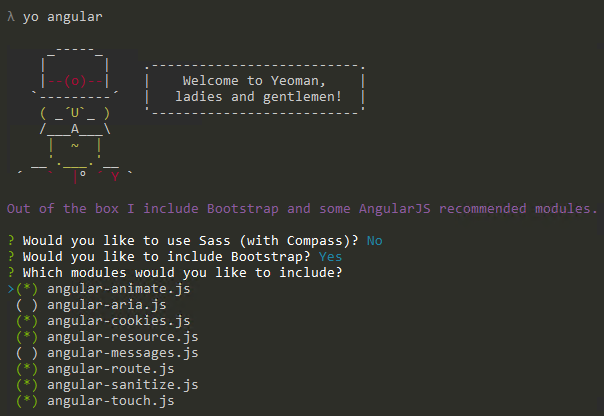
\includegraphics[width=.4\textwidth]{img/tp1_parte2/0-instalacionConYeoman}
  \caption{Confifuración inical de Yeoman}
  \label{yeomanInstall}
\end{figure}

Una vez terminada la configuración de Yeoman, en la carpeta del proyecto tendremos el esqueleto necesario para empezar a trabajar. En la  \textbf{Figura \ref{scaffold}} podemos ver cuales son los directorios principales, siendo estos \textbf{\textit{app}} donde se encuentran las imagenes, los controladores y las vistas y el directorio \textbf{\textit{test}} donde se encuentran los test respectivos para cada uno de los controladores.

\begin{figure}[h]
  \centering
  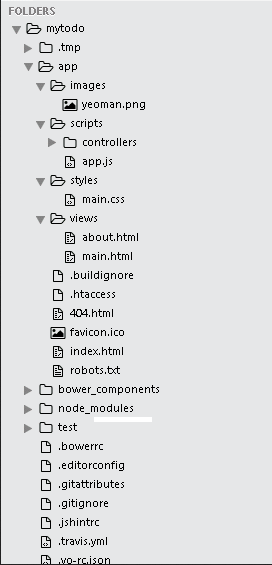
\includegraphics[width=.4\textwidth]{img/tp1_parte2/0-scaffold}
  \caption{scaffold de la aplicación inicial}
  \label{scaffold}
\end{figure}

\subsection{Diagrama de clases tentativo}
{\correccionTexto
En la \textbf{Figura \ref{2-modelo_datos_general}} se presenta el diagrama de clases tentativo, dicho diagrama  será utilizado como base a lo largo de los futuros sprint a desarrollar y posee un alcance limitado el cual se irá modificando a medida que se profundice en los temas.

Para realizar este diagrama se utilizaron los user stories definidos con anterioridad y el relevamiento que se ha realizado hasta el momento, pero como se dijo anterirormente, muchos de los temas serán profundizados en cada Sprint.
}

\begin{correccionSidewaysFigure}
  \centering
  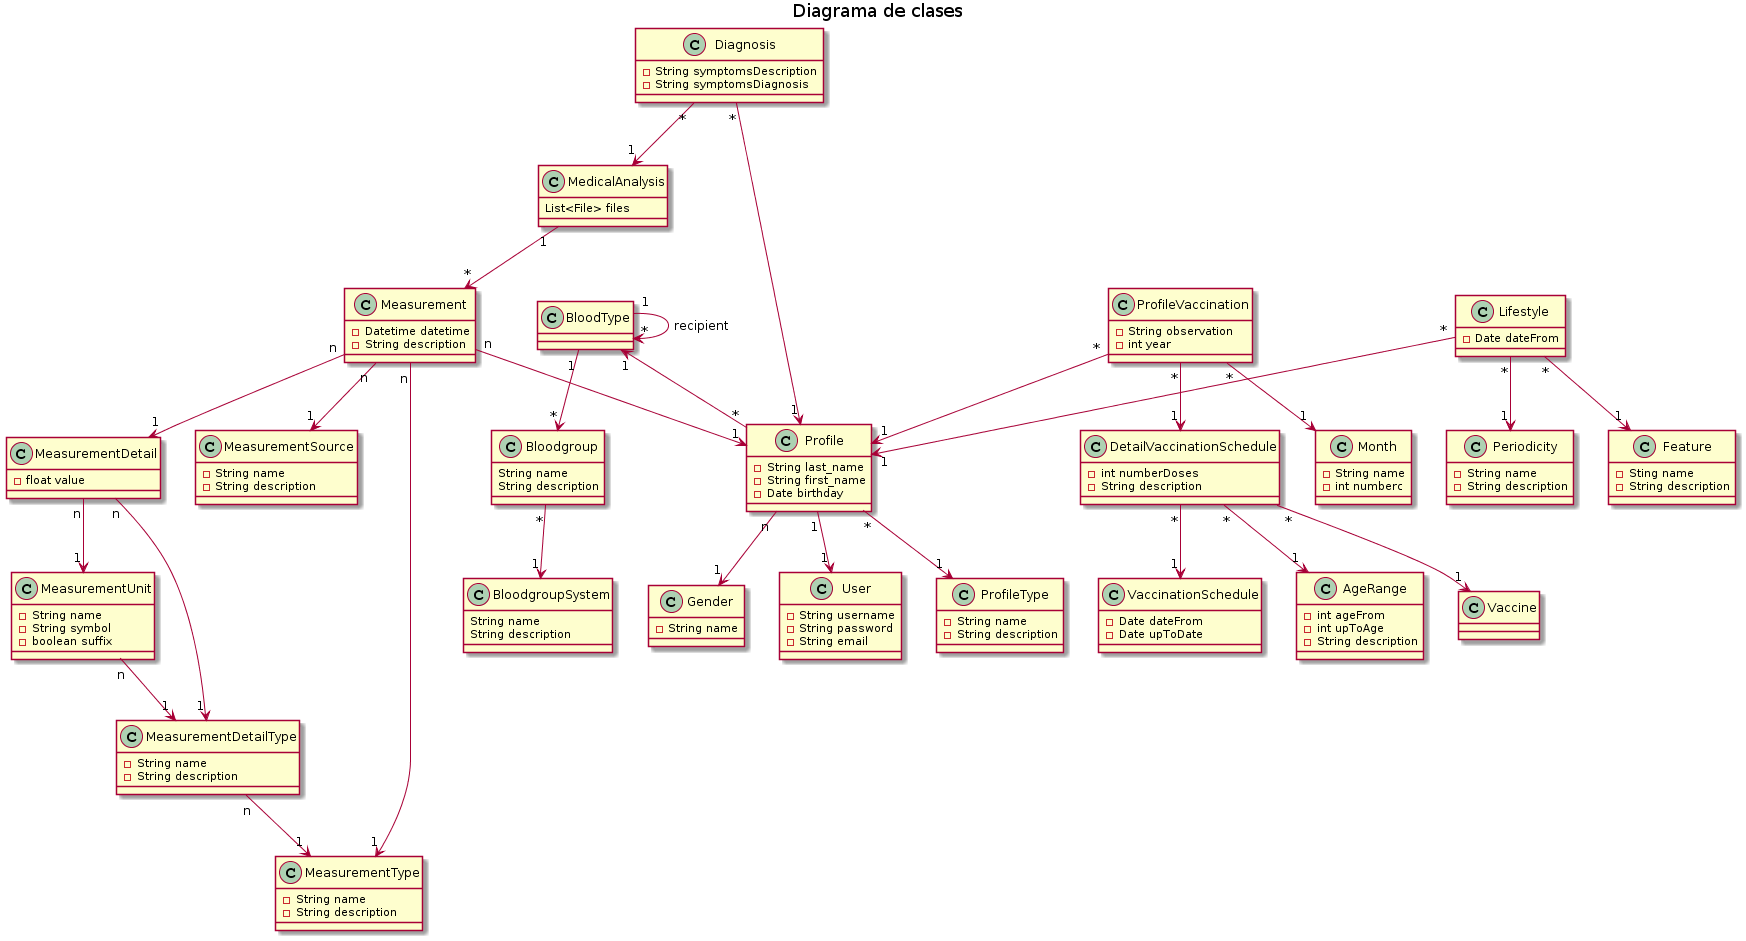
\includegraphics[width=0.9 \textwidth]{img/tp1_parte2/0-DiagramaClasesGeneral}
  \caption{Modelo de datos General}
  \label{2-modelo_datos_general}
\end{correccionSidewaysFigure}


\clearpage % Lo hice para que la imagen del scaffold no me quede tan abajo